\section{Transfer Function and Compensator Design}
\subsection{Transfer Function Derivation}

In the transfer function derivation, we are going to use averaging method. [3]

In the forward converter below Figure \ref{forward1} we can observe the forward converter. Here, we are starting with defining the $x_1 = i_L$ and $x_2 = v_c$. These two states will be taken into account from now on.

\begin{center}
\begin{figure}[H]
\centering
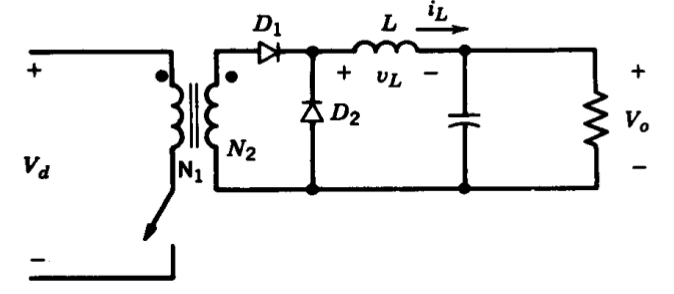
\includegraphics [width=12 cm, height= 6 cm]{forward.png}
\caption{Forward Converter Topology}
\label{forward1}
\end{figure}
\end{center}

When we use the averaging method. It is important to use the switch ON and switch OFF models of the converter. Below, we can observe these models in Fig. \ref{fig:switch}.

\begin{figure}[H]
\centering
\begin{subfigure}{7 cm}
  \centering
  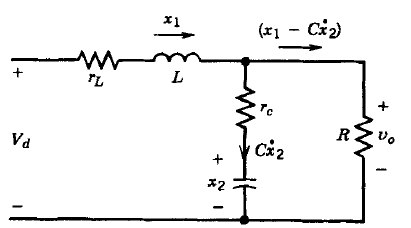
\includegraphics[width=7 cm]{Figs/switchON.PNG}
  \caption{Switch ON}
  \label{fig:input_current_48}
\end{subfigure}%
\begin{subfigure}{7 cm}
  \centering
  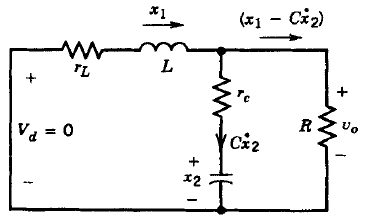
\includegraphics[width=7 cm]{Figs/switchOFF.PNG}
  \caption{Switch OFF}
  \label{fig:inductor_current_48}
\end{subfigure}
\caption{Forward converter averaging models switch on (a) and switch off (b)}
\label{fig:switch}
\end{figure}

In the first model, we can write that: assuming turn ratio is N.

\begin{equation}
    -NV_d + r_L i_L + L \Dot{i_L} + R(i_L - C\Dot{v_C}) = 0
\end{equation}

and 

\begin{equation}
    -v_c + C r_c \Dot{v_C} + R(i_L - C\Dot{v_c}) = 0
\end{equation}

Basically, when switch is on if we call this state space representation number 1, then it will have following structure:

\begin{equation}
\begin{bmatrix}
\Dot{i_L} \\ \Dot{v_C}
\end{bmatrix}
=
\begin{bmatrix}
 -\dfrac{Rr_c + Rr_L + r_C r_L}{L(R + r_C)} & -\dfrac{R}{L(R + r_C)} \\
 \dfrac{R}{C(R + r_C)} & -\dfrac{1}{C(R + r_C)} 
\end{bmatrix}
\begin{bmatrix}
i_L \\ v_C
\end{bmatrix}
+
\begin{bmatrix}
\dfrac{1}{L} \\ 0
\end{bmatrix}
NV_d
\end{equation}

Let us call this state space representation as

$$ \Dot{x} = A_1 x + B_1 u$$

When the switch is off, we can write following equations:
\begin{equation}
  r_L i_L + L \Dot{i_L} + R(i_L - C\Dot{v_C}) = 0  
\end{equation}
and

\begin{equation}
    -v_c + C r_c \Dot{v_C} + R(i_L - C\Dot{v_c}) = 0
\end{equation}

Switch is off, if we call this state space representation number 2, then it will have following structure:

\begin{equation}
\begin{bmatrix}
\Dot{i_L} \\ \Dot{v_C}
\end{bmatrix}
=
\begin{bmatrix}
 -\dfrac{Rr_c + Rr_L + r_C r_L}{L(R + r_C)} & -\dfrac{R}{L(R + r_C)} \\
 \dfrac{R}{C(R + r_C)} & -\dfrac{1}{C(R + r_C)} 
\end{bmatrix}
\begin{bmatrix}
i_L \\ v_C
\end{bmatrix}
\end{equation}

Let us call this state space representation as

$$ \Dot{x} = A_2 x$$

As we can easily see $A_1 = A_2$ and more importantly $B_2 = 0$. Therefore averaging is much easier in this topology. Now, we can say that
\begin{equation}
    A = A_1D + A_2(1-D) = A_1
\end{equation}
and

\begin{equation}
    B = B_1D
\end{equation}

Let's derive the output. If we are to define the output as $v_o$ then we can write that

\begin{equation}
    v_o = R(i_L - C\Dot{v_C})
\end{equation}

in state space form for both switch on and off cases

\begin{equation}
    v_o = \begin{bmatrix}
    \dfrac{R r_c}{R+r_C}i_L & \dfrac{R}{R+r_c}v_C
    \end{bmatrix}
\end{equation}

To simplify these state space representations, we will follow a simple approach. In our circuitry, $r_c = 3 m\ohm$, $r_L = 60 m\ohm$ where $R = 4.7 \ohm$. Starting from this point, apparently, we can assume that
\begin{equation}
R \gg (r_C + r_L)
\end{equation}

so A is simplified as:

\begin{equation}
    A = \begin{bmatrix}
 -\dfrac{r_c + r_L}{L} & -\dfrac{1}{L} \\
 \dfrac{1}{C} & -\dfrac{1}{CR} 
\end{bmatrix}
\end{equation}

B is simplified as:

\begin{equation}
    B = \begin{bmatrix} 
 \dfrac{1}{L} \\ 0 
\end{bmatrix}
D
\end{equation}

C is simplified as:

\begin{equation}
C =
    \begin{bmatrix}
    r_C & 1
    \end{bmatrix}
\end{equation}

Now, we need to introduce small signal perturbations to the system.
\begin{equation}
  d = D + \Tilde{d}  
\end{equation}
\begin{equation}
  v_o = V_o + \Tilde{v_o}  
\end{equation}
and 
\begin{equation}
  x = X + \Tilde{x}  
\end{equation}

Now the equation becomes:

\begin{equation}
    \Tilde{\Dot{x}} = A\Tilde{x} + B N V_d \Tilde{d}
\end{equation}

and 

\begin{equation}
    \Tilde{v_o} = C\Tilde{x}
\end{equation}

when we use the laplace transformation:

\begin{equation}
    \Tilde{x}(s) = [sI-A]^{-1}(B_1 V_d)\Tilde{d(s)}
\end{equation}

So, output to control transfer function can be written as:

\begin{equation}
\dfrac{\Tilde{v_o}(s)}{\Tilde{d}(s)} = C[sI-A]^{-1} B N V_d    
\end{equation}

\begin{equation}
   \dfrac{\Tilde{v_o}(s)}{\Tilde{d}(s)} = NV_d \dfrac{1 + sr_C C}{LC (s^2 + s (\dfrac{1}{RC} + \dfrac{(r_c + r_L)}{L}) + \dfrac{1}{LC}) }
\end{equation}

\subsection{Bode Plot of the Forward Converter}

Let's have a look at to the bode plot of the forward converter. In the ideal case where capacitor and inductor resistance does not exist, the transfer function can be simplified as:

\begin{equation}
   \dfrac{\Tilde{v_o}(s)}{\Tilde{d}(s)} = NV_d \dfrac{1}{LC (s^2 + s \dfrac{1}{RC} + \dfrac{1}{LC}) }
\end{equation}

When we obtain its bode plot using Matlab, the resulting graph is below Fig \ref{fig:bode_24}. Also, below we have non-ideal bode plots Figure \ref{fig:bode_non_24} and \ref{fig:bode_non_48}

\begin{figure}[H]
\centering
\begin{subfigure}{7 cm}
  \centering
  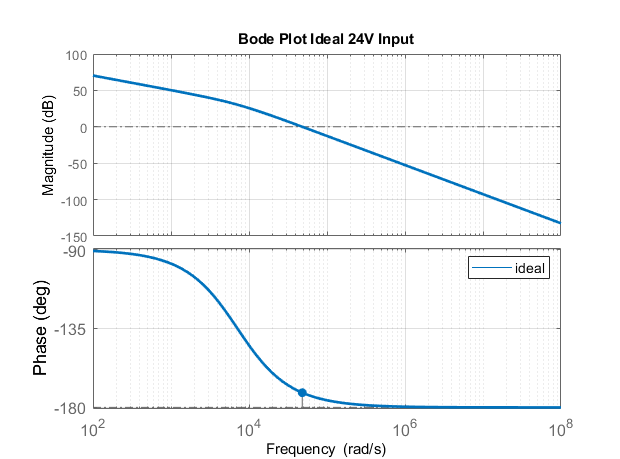
\includegraphics[width=7 cm]{Figs/bode_24_ideal.png}
  \caption{Ideal}
  \label{fig:bode_24}
\end{subfigure}%
\begin{subfigure}{7 cm}
  \centering
  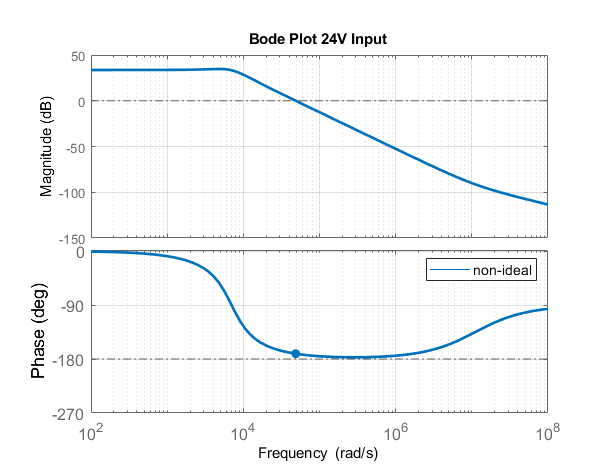
\includegraphics[width=7 cm]{Figs/bode_24_non.png}
  \caption{Non-ideal}
  \label{fig:bode_non_24}
\end{subfigure}
\caption{Bode plot with input 24V ideal (a) and non-ideal (b)}
\label{fig:bode24}
\end{figure}

\begin{figure}[H]
\centering
\begin{subfigure}{7 cm}
  \centering
  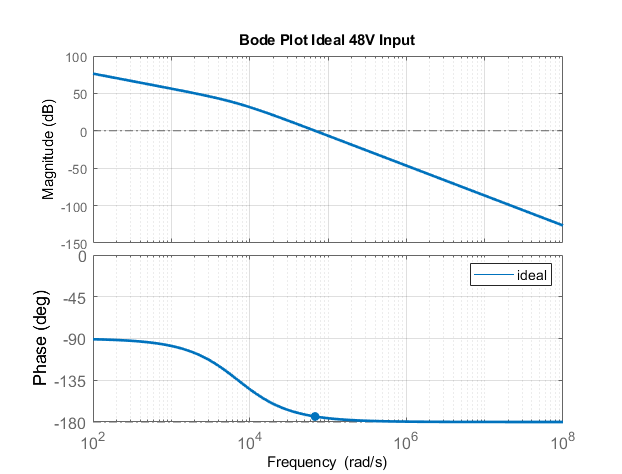
\includegraphics[width=7 cm]{Figs/bode_48_ideal.png}
  \caption{Ideal}
  \label{fig:bode_48}
\end{subfigure}%
\begin{subfigure}{7 cm}
  \centering
  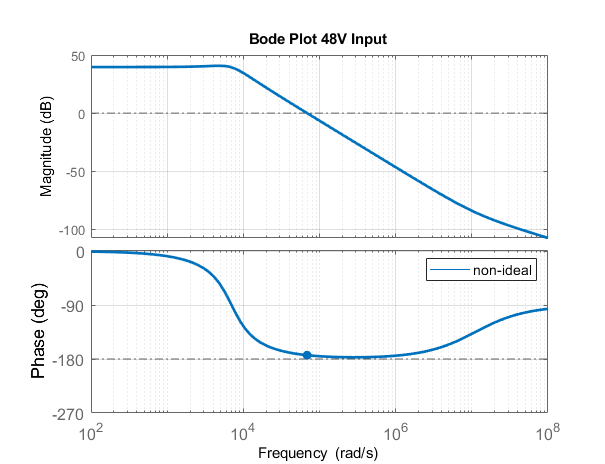
\includegraphics[width=7 cm]{Figs/bode_48_non.png}
  \caption{Non-ideal}
  \label{fig:bode_non_48}
\end{subfigure}
\caption{Bode plot with input 48V ideal (a) and non-ideal (b)}
\label{fig:bode48}
\end{figure}


At the worst case, the input is 48V. Below, we can observe the phase margin of 48V input bode plot with all non-idealities. Figure \ref{bode_big_48}

\begin{center}
\begin{figure}[H]
\centering
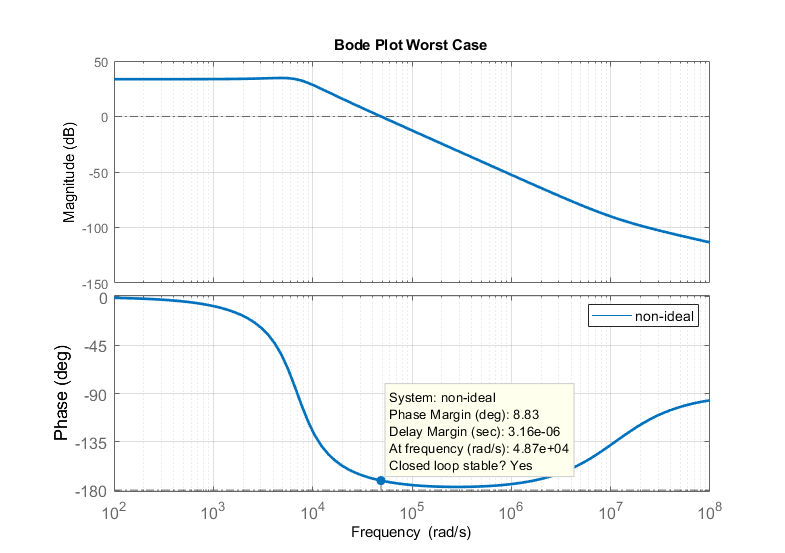
\includegraphics [width=14 cm]{bode_worst.png}
\caption{Bode plot of forward converter, worst case}
\label{bode_big_48}
\end{figure}
\end{center}

As we can follow, forward converter is a stable converter with a very small phase margin. Nevertheless, we need to design a compensator that will boost the phase of the converter so that we can operate in stable region with considerable speed. Now, we are going to design a compensator to make this system more stable. Also, we want to operate in constant output voltage!

\subsection{Compensator Design}

Basically, a forward converter and a boost converter have similar transfer functions. Its difference is that the input voltage reflects with a turn ratio, nonetheless, the rest is almost same. Therefore, we can apply a buck compensator for the forward converter, and make it work! We are applying the procedure in the given note. [4]

Firstly, it is important to see that we need to boost our phase margin due to increase stability. An operation around 40-70\degree will be enough for our operation. It is obvious that we need a type three compensator to boost our phase margin. Also, if we calculate the frequencies of the circuitry we can easily see that:

\begin{equation}
    F_{esr} = \dfrac{1}{2 \pi R_{ESR} C_o} = 1.77 MHz
\end{equation}
\begin{equation}
    F_{LC} = \dfrac{1}{2 \pi \sqrt{LC}} = 1.11 kHz
\end{equation}
\begin{equation}
    F_{0} = \dfrac{f_s}{10} = 2.5 kHz
\end{equation}

Basically, we can see that:

\begin{equation}
    F_{LC} < F_{O} < F_S/2 < F_{ESR}
\end{equation}

We should use Type-III Compensator! Also, it is very convenient because we have used a ceramic capacitor at the output!

\begin{wrapfigure}{r}{0.5\textwidth}
  \vspace{-20pt}
  \begin{center}
    \includegraphics[width=0.4\textwidth]{Figs/compansator_model.PNG}
  \end{center}
  \vspace{-20pt}
  \caption{Snubber Layout}
  \label{Snubberlayout}
  \vspace{-10pt}
\end{wrapfigure}

At this point, we need to introduce the schematic of compensator! This compensator consists of 3 poles and 2 zeros. One pole is an integrator, which makes the steady state error zero. So, at the low frequencies we have a $-90 \degree$ boost shift. However, at the proper locations we have a phase boost up to $90 \degree$ theoretically. Here, an important factor is that, at the oscillator we are using $1.8V$ oscillator voltage with the frequency of $25kHz$. It is significant that, we should have a duty cycle limit of $D_{max} = 0.5$. Nonetheless, we can apply further duty cycles, the third winding will be a problem. So, $V_{ref}$ must be maximum of $0.9V$ for operation.

\begin{equation}
    V_{ref} = 0.9V
\end{equation}

Here is the transfer function:

\begin{equation}
    H(s) = \dfrac{(1+sR_{C1}+C_{C1})(1+sC_{f3}(R_{f1}+R_{f3}))}{sR_{f1}(C_{C1}+C_{C2})(1+sR_{C1}(\dfrac{C{C1}C_{C2}}{C{C1}+C_{C2}})(1+sR_{f3}C_{f3}}
\end{equation}

\begin{equation}
    F_{Z1} = \dfrac{1}{2\pi R_{C1}C_{C1}}
\end{equation}
\begin{equation}
     F_{Z2} = \dfrac{1}{2\pi C_{f3}(R_{f1}+R_{f3})}
\end{equation}
\begin{equation}
    F_{p1} = 0
\end{equation}
\begin{equation}
    F_{p2}   = \dfrac{1}{2\pi R_{f3}C_{f3}}
\end{equation}
\begin{equation}
    F_{p3}   = \dfrac{1}{2\pi R_{C2}C_{C2}}
\end{equation}

Now, it is important to decide the pole and zero locations in order to have a proper compensator. We place the $F_{p3}$ to the $F_s/2$ to have a low-pass structure, and to eliminate the ripples above the switching frequency. 
$$F_{p3} = \dfrac{F_s}{2} = 12.5kHz$$
Now, we need to design the lead-compensator part. As we know, a type-3 compensator can boost up the phase margin maximum of 90 \degree. However, in practical it is maximum 80 \degree. A phase-lead compensator consists of one pole and one zero. This compensator must be located at the crossover frequency to boost up the phase margin. We should use following formulas:

$$ F_{Z2} = F_0  \sqrt{\dfrac{1-\sin{\theta} }{{1+\sin{\theta}}}}$$
$$ F_{p2} = F_0  \sqrt{\dfrac{1+\sin{\theta} }{{1-\sin{\theta}}}}$$

Since, my phase margin is negative right now, i should get the maximum of phase shift. We put the $\theta$ at limit, $\theta = 80 \degree$. Since, i selected the crossover frequency as $F_s/10$ the zero of the lead-compensator will result in increment of the gain. We were expecting an increase in gain in the lead-compensator part.

$$ F_{Z2} = 418 Hz$$

$$ F_{p2} = 28.38 kHz$$

We chose the second zero before the first one in order not to have decrements in the gain. It is significant to sustain  gain level. We chose

$$F_{Z1} = \dfrac{F_{Z2}}{2} = 210 Hz $$

After this point, we need to select a proper capacitor for $C_{f3}$, i choose this capacitor value as $2.2 nF$.

$$R_{f3} \approx 2.55k\ohm$$

then

$$ R_{f1} \approx 170k\ohm $$

using this the data given in the application note:

$$ R_{C1} = \dfrac{2\pi F_0 L_o C_o V_{osc}}{V_{in}C_{f3}}$$

There, since it is a forward converter the capacitor and inductor values are what they are!

$$ R_{C1} \approx 5.46k \ohm $$

using $R_{C1}$

$$C_{C1} = 140 nF $$

$$C_{C2} = 2.33 nF $$


$$ R_{f2} = \dfrac{R_{f1}V_{ref}}{V_{out}-V_{ref}} = 10.9k\ohm$$


\begin{figure}[H]
\centering
\begin{subfigure}{7 cm}
  \centering
  \includegraphics[width=7 cm]{Figs/conv.png}
  \caption{Plant}
  \label{fig:input_current_24_com}
\end{subfigure}%
\begin{subfigure}{7 cm}
  \centering
  \includegraphics[width=7 cm]{Figs/comp.png}
  \caption{Compensator}
  \label{fig:inductor_current_24_com}
\end{subfigure}
\caption{Forward converter plant (a) and compensator (b) bode plot}
\label{fig:current_24}
\end{figure}

\begin{center}
\begin{figure}[H]
\centering
\includegraphics [width=14 cm]{open.png}
\caption{Open-loop bode plot}
\label{Output24com}
\end{figure}
\end{center}

In the resultant bode plot, we can see that the phase margin is boosted up to 55\degree and the bandwidth is very convenient. Let's construct the LTSpice model of this compensator.

\begin{center}
\begin{figure}[H]
\centering
\includegraphics [width=15 cm]{compansator_schematic.png}
\caption{Forward converter with compensator}
\label{CompensatorSchema}
\end{figure}
\end{center}

To simulate the line regulation and load regulation, first we increased the input from 24V to 48V, and observed the output. Below in the Fig \ref{inputC} we can see the output waveform. We changed the output from 24V to 48V at 2ms.

\begin{center}
\begin{figure}[H]
\centering
\includegraphics [width=12 cm]{inputChange}
\caption{Input change line regulation}
\label{inputC}
\end{figure}
\end{center}

 Fig \ref{inputC} shows that the line regulation is below 2\%, the output goes back to 15V after the line regulation, and it continues its operation. The transient is stable and we observe an overshoot around the regulation time. Therefore, our compensator design is valid. Let's now look at the load regulation.
 
 \begin{center}
\begin{figure}[H]
\centering
\includegraphics [width=12 cm]{loadTen}
\caption{Load change, load regulation}
\label{inputT}
\end{figure}
\end{center}

Again, in the Fig \ref{inputT}, we can observe that the load regulation is less than 2\%. In this case at 3ms, we increased the load from 0.32A, to 3.2A (full load) and we can see that after the transient our load regulation is as expected. We have some overshoot during the transient.

In this part, we designed our compensator and now we have a closed loop operation. The converter is stable and line, load regulations are below 2 \%. 
 
 













